\subsection{Unified Modellig Language}
En af de anvendte sprog indenfor objektorienteret programmering er standarden Unified Modelling Language (UML). Ud fra denne standard anvendes modeller til at visualisere struktur og egenskaber af systemet. Derudover relaterer metoderne til analyse og design af systemet. Modeller til at visulisere egenskaber er blandt andet use case diagrammer og aktivitetsdiagrammer. Til visualisering af struktur anvendes blandt andet klassediagrammer \cite{Fowler2004, Williams2004}.


\subsubsection{Use case diagrammer} 
Use case diagrammer benyttes til at illustrere aktørernes interaktion med et system samt, hvordan forskellige use cases interagerer mellem hinanden. Dertil er use case diagrammet med til at repræsentere funktionelle krav for systemet. \cite{Williams2004} Et eksempel på et use case diagram ses af \autoref{fig:use_case}.

\begin{figure} [H]
\centering
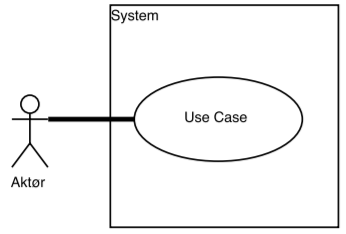
\includegraphics[width=0.5\textwidth]{figures/USE_CASE2}
\caption{Simpelt use case diagram.}
\label{fig:use_case}
\end{figure}

\noindent
Af \autoref{fig:use_case} ses aktørens interaktion med use case visualiseret som en streg mellem de to. I et use case diagram vil aktøren definere en person, der kan tilgå systemets funktionaliteter. Dette kan eksempelvis være en person, rolle, objekt eller en anden given genstand. Hertil vil den enkelte use case beskrive en handling eller funktionalitet i systemet.\cite{Fowler2004, Williams2004}


\subsubsection{Aktivitetsdiagrammer} 
Aktivitetsdiagrammer anvendes til at beskrive hvad der sker i programmet, herunder proceduremæssig logik, business processer og arbejdsflow. Aktiviteter kan opdeles i subaktiviteter eller metoder. Subaktiviteter vil fremgå af diagrammet ved et rivesymbol, mens metoder vil fremgå ved syntaxen klasse-navn::metode-navn. Aktivitetsdiagrammer fortæller ikke hvem der udføre aktiviteten, hertil kan der anvendes skillevæge, som viser, hvilken aktivitet en klasse eller organisation tilhører. Et simpelt aktivitetsdiagram fremgår af \autoref{fig:aktivitetsdiagram}.









 Hvert aktivitetsdiagram starter ved en initial node, som 
påkalder et program eller en rutine.



Aktiviteter kan også svare på signaler eksempelvis tid. 



Et signal angiver
at aktiviteten modtager en begivenhed fra en ekstern proces. Dette indikerer, at
aktiviteten lytter konstant til Valgte signaler, og diagrammet definerer, hvordan den
aktivitet reagerer.
I tilfælde af


slutter med en final. Derudover kan aktivitet 
%Til at beskrive komplekse use cases eller klassemetoder anvendes aktivitetsdiagrammer. Dette giver overblik over flowet gennem de forskellige aktiviteter i den givne funktion eller metode. \cite{Fowler2004}    

%Såfremt der i et aktivitetsdiagram anvendes et 'brille' symbol, indikerer dette at den aktivitet i sig selv er kompleks og er beskrevet i et særskilt aktivitetsdiagram.  

\subsubsection{Klassediagrammer}
Klassediagrammer anvendes som redskab til at designe og give overblik over de forskellige klasser. Hertil vil relationerne mellem de forskellige klasser blive tydeliggjort ved anvendelse af tilhørende symbolisering: nedarvning, association %aggregation, composition 
med mere. Som det ses af \autoref{fig:klassediagram} beskrives hver klasse ud fra et unikt klassenavn, hvor der yderligere kan tildeles attributter og metoder til den givne klasse.\cite{Fowler2004} 

\begin{figure} [H]
\centering
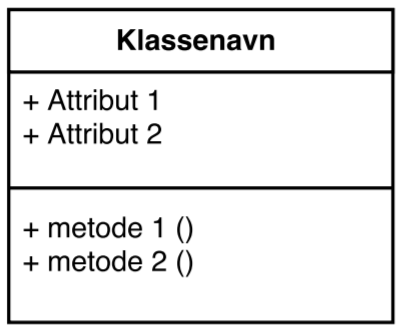
\includegraphics[width=0.5\textwidth]{figures/klassediag}
\caption{}
\label{fig:klassediagram}
\end{figure}